\documentclass[11pt, a4paper]{article}

\usepackage{amsmath, amsfonts, amssymb, amstext, amscd, amsthm, bbm, CJKutf8, color, dsfont, enumerate, float, graphicx, hyperref, lipsum, makeidx, mathrsfs, mathtools, marvosym, soul, stmaryrd, url, verbatim, xcolor, xfrac}
\usepackage[left=2cm,top=2cm,right=2cm,bottom=2cm,bindingoffset=0cm]{geometry}
\hypersetup{
    colorlinks=true,
    linkcolor=black!50!red,
    urlcolor=black!50!red
}
\allowdisplaybreaks

\newenvironment{subproof}[1][Proof]
    {\proof[#1]\leftskip=1cm\rightskip=1cm}
    {\endproof}

%theorems with custom numbering
%\newtheorem{innerthm}{Theorem}
%\newenvironment{thm}[1]
    %{\renewcommand\theinnerthm{#1}\innercustomthm}
    %{\endinnerthm}

\newtheorem{theorem}{Theorem}
\newtheorem{lemma}{Lemma}
\newtheorem{proposition}{Proposition}
\newtheorem{corollary}{Corollary}
\newtheorem{claim}{Claim}
\newtheorem{conjecture}{Conjecture}
\newtheorem{justification}{Justification}
\newtheorem{definition}{Definition}
\newtheorem*{remark}{Remark}
\newtheorem*{note}{Note}

\renewcommand{\restriction}[1]{\downharpoonright_{#1}}
\renewcommand{\qedsymbol}{\sc q.e.d.}
\renewcommand{\leq}{\leqslant}
\renewcommand{\geq}{\geqslant}
\renewcommand{\and}{~\wedge~}
\newcommand{\defn}{\coloneqq}
\newcommand{\disj}{~\vee~}
\newcommand{\xor}{~\oplus~}
\newcommand{\divides}{~|~}
\newcommand{\given}{~\middle|~}
\newcommand{\suchthat}{~\middle|~}
\newcommand{\contradiction}{~\text{\Large \Lightning}}
\newcommand{\conj}[1]{\overline{#1}}
\newcommand{\mean}[1]{\overline{#1}}
\newcommand{\integral}[1]{\smashoperator{\int_{#1}}}
\newcommand*\diff{\mathop{}\!\mathrm{d}}
\newcommand{\E}[1]{\mathbb{E}\sqparens*{#1}}
\newcommand{\Esub}[2]{\mathbb{E}_{#1}\sqparens*{#2}}
\newcommand{\var}[1]{\mathrm{Var}\parens*{#1}}
\newcommand{\cov}[2]{\mathrm{Cov}\parens*{#1, #2}}
\newcommand{\der}[2]{\frac{\diff{#1}}{\diff{#2}}}
\newcommand{\dern}[3]{\frac{\diff^{#3}{#1}}{\diff{#2}^{#3}}}
\newcommand{\derm}[3]{\frac{\diff^{#3}{#1}}{\diff{#2}}}
\newcommand{\prt}[2]{\frac{\partial{#1}}{\partial{#2}}}
\newcommand{\prtn}[3]{\frac{\partial^{#3}{#1}}{\partial{#2}^{#3}}}
\newcommand{\prtm}[3]{\frac{\partial^{#3}{#1}}{\partial{#2}}}

\DeclareMathOperator{\lcm}{lcm}
\DeclareMathOperator*{\argmin}{arg\!\min}
\DeclareMathOperator*{\argmax}{arg\!\max}

\let\originalleft\left
\let\originalright\right
\renewcommand{\left}{\mathopen{}\mathclose\bgroup\originalleft}
\renewcommand{\right}{\aftergroup\egroup\originalright}
\newcommand{\zh}[1]{\begin{CJK}{UTF8}{gbsn}#1\end{CJK}}
\newcommand{\jp}[1]{\begin{CJK}{UTF8}{gbsn}#1\end{CJK}}


\DeclarePairedDelimiterX \inner[2]{\langle}{\rangle}{#1,#2}
\DeclarePairedDelimiterX \braket[2]{\langle}{\rangle}{#1 \delimsize\vert #2}
\DeclarePairedDelimiter \bra{\langle}{\rvert}
\DeclarePairedDelimiter \ket{\lvert}{\rangle}
\DeclarePairedDelimiter \abs{\lvert}{\rvert}
\DeclarePairedDelimiter \norm{\lVert}{\rVert}
\DeclarePairedDelimiter \set{\lbrace}{\rbrace}
\DeclarePairedDelimiter \seq{\langle}{\rangle}
\DeclarePairedDelimiter \parens{(}{)}
\DeclarePairedDelimiter \sqparens{[}{]}

\begin{document}
\begin{center}
    \textsc{\huge Monte Carlo Methods}\\
    \textsc{\Large Homework 4}\\
\end{center}
\begin{flushright}
    Daniel Gonzalez\\
    $9$\textsuperscript{th} of April, $2019$
\end{flushright}

\begin{enumerate}
    \item \label{1}
        {\it Consider the Bernoulli probability mass function $f(x) \defn p^x(1 - p)^{1 - x}$ for $x \in \set*{0, 1}$.
        Find the corresponding tilted probability mass function $f_t(x)$.
        Is $f_t(x)$ a Bernoulli mass function?}

        The twisted probability mass function is given by $f_t(x) \defn \frac{e^{tx}f(x)}{M(t)}$ with $M(t) \defn \E{e^{tX}}$ where $X \sim \text{Bernoulli}(p)$.
        We can compute $M(t) = \E{e^{tX}} = \sum_{x = 0}^{1}e^{tx}f(x) = 1 - p + e^tp$.
        This gives us the following form for the twisted function:
        \begin{align*}
            f_t(x) &= \frac{e^{tx}f(x)}{M(t)}
            = \frac{e^{tx}p^x(1 - p)^{1 - x}}{1 - p + e^tp}
            =
            \begin{cases}
                \displaystyle\frac{1 - p}{1 - p + e^tp} &\text{ if } x = 0\\
                \\
                \displaystyle\frac{e^tp}{1 - p + e^tp}  &\text{ if } x = 1.
            \end{cases}
        \end{align*}
        If we let $q \defn \frac{e^tp}{1 - p + e^tp}$, we can observe that $1 - q = 1 - \frac{e^tp}{1 - p + e^tp} = \frac{1 - p}{1 - p + e^tp}$,
        and therefore $f_t(x) = q^x(1 - q)^{1 - x}$ for $x \in \set*{0, 1}$, so that $f_t(x)$ is indeed a Bernoulli probability mass function.
    \item \label{2}
        {\it Let $X$ be a random variable such that $0 \leq X \leq a$ for some $a \in \mathbb{R}$.}
        \begin{enumerate}
            \item \label{2a}
                {\it Show that $\E{X^2} \leq a\E{X}$.}
                \begin{proof}
                    Given a measure space $\parens*{\Omega, \mathcal{F}, \mu}$ and two measurable functions $f: \Omega \to \mathbb{R}$ and $g: \Omega \to \mathbb{R}$
                    such that $f(\omega) \leq g(\omega)$ for all $\omega \in \Omega$, we know that
                    \begin{equation*}
                        \int_{\Omega}f\diff{\mu} \leq \int_{\Omega}g\diff{\mu}.
                    \end{equation*}
                    In the case that $\mu$ is a probability measure and $f$ and $g$ are random variables, this gives us $\E{f} \leq \E{g}$.
                    Now, since $0 \leq X \leq a$, we know that $X^2 \leq aX$. Applying the above property gives us the conclusion $\E{X^2} \leq \E{aX} = a\E{X}$.\\
                \end{proof}
            \item \label{2b}
                {\it Show that $\var{X} \leq \E{X}\parens*{a - \E{X}}$.}
                \begin{proof}
                    Using \ref{2a}, we have
                    \begin{equation*}
                        \var{X} = \E{X^2} - \E{X}^2
                        \leq a\E{X} - \E{X}^2
                        = \E{X}\parens*{a - \E{X}}.
                    \end{equation*}
                \end{proof}
            \item \label{2c}
                {\it Show that $\var{X} \leq \sfrac{a^2}{4}$.}
                \begin{proof}
                    Let $c \defn \frac{\E{X}}{a}$ and observe that, from \ref{2b}, we can write
                    \begin{equation*}
                        \var{X} \leq \E{X}\parens*{a - \E{X}} = a^2\frac{\E{X}}{a}\parens*{1 - \frac{\E{X}}{a}} = a^2c(1 - c).
                    \end{equation*}
                    Since $0 \leq X \leq a$, we know that $0 = \E{0} \leq \E{X} \leq \E{a} = a$, and so $0 \leq c \leq 1$.
                    To find an upper bound on $c$, we can maximize $\varphi(x) \defn x(1 - x) = x^2 - x$
                    in the interval $[0, 1]$ by finding the critical points of its derivative.
                    Clearly, $\varphi'(x) = 2x - 1$ has only one root at $x = \sfrac{1}{2}$.
                    Evaluating $\varphi$ at the critical points $x \in \set*{0, \sfrac{1}{2}, 1}$,
                    we find that its maximum value is $\varphi\parens*{\sfrac{1}{2}} = \sfrac{1}{4}$.
                    Therefore, we have $c(1 - c) \leq \sfrac{1}{4}$.
                    We can then conclude that
                    \begin{equation*}
                        \var{X} \leq a^2c(1 - c) \leq \sfrac{a^2}{4}.
                    \end{equation*}
                \end{proof}
        \end{enumerate}
    \item \label{3}
        {\it In Chapter $4$, we discussed a control variate approach to pricing arithmetic Asian call options using geometric Asian call options as a control.
        Write a code to implement the control variate method using low-discrepancy sequences
        and construct a table of results using RQMC with the same parameters as the one given in the lecture notes.}

        We implemented the pricing strategy described using random-shift Halton sequences
        in the \texttt{control\_variates.jl} file in \href{https://julialang.org}{Julia}.
        The na\"ive pricing strategy was implemented by \texttt{crude($\dots$)},
        and the control-variate method was implemented by \texttt{control($\dots$)}.
        The \texttt{estimate(num)} then runs each of the pricing strategies $\texttt{num} = 50$ many times

        In Table \ref{tab:asian} below, we summarize the results of the pricing strategies using the given parameters
        $r = 0.035$, $\sigma = 0.2$, $T = 1$, $K = 90$, $S_0 = 100$, $n = 20$ from the notes.
        The estimated crude RQMC price of the arithmetic Asian option with $N = 100,000$ is $12.25593681091458$,
        while the estimated control RQMC price is $12.258116304664235$ with the same $N$.
        The ``true" price of the Asian option is given as $11.81958519819731$ in the notes.
        \begin{table}[H]
            \centering
            \caption{Sample Variance of $50$ Price Estimates}
            \begin{tabular}{|r|l|c|c|c|c|} \hline
                                & $N = 10,000$              & $N = 50,000$              \\ \hline
                Crude RQMC      & $3.874 \times 10^{-5}$    & $5.514 \times 10^{-6}$    \\ \hline
                Control RQMC    & $3.989 \times 10^{-5}$    & $2.272 \times 10^{-6}$    \\ \hline
            \end{tabular}
            \label{tab:asian}
        \end{table}
        As we can see, the variances of both methods are comparable and both experience an order-magnitude reduction in variance as the number of sample paths is increased,
        though the control-variate method demonstrates about a factor of $2$ reduction in the variance over the crude method when $N = 50,000$.
        They are both on the same magnitude as the variance given in the notes for the control MC price estimates,
        although the actual estimated price is further off for both of them than the prices predicted by the MC methods,
        which are given as $12.09638460$ and $12.09966098$ in the notes for the crude and control approaches respectively.
        
    \item \label{4}
        {\it In the following, we will use Monte Carlo simulation to estimate $\theta = \E{e^{U}} = \int_{0}^{1}e^x\diff{x}$.}
        \begin{enumerate}
            \item \label{4a}
                {\it What is the sample mean estimator and the antithetic variates estimator for $\theta$?
                Find the variance of these two estimators,
                and find how much variance reduction is achieved by the antithetic variates estimator over the sample mean estimator.}

                If we let $U \sim U(0, 1)$, then the sample mean estimator for $\theta$ is given by
                \begin{equation*}
                    \mean{\theta} = e^U,
                \end{equation*}
                and the antithetic variates estimator is given by
                \begin{equation*}
                    \mean{\theta}_a = \frac{e^U + e^{1 - U}}{2}.
                \end{equation*}
                The variance of $\mean{\theta}$ is then given by
                \begin{align*}
                    \var{\mean{\theta}} &= \E{e^{2U}} - \E{e^U}^2\\
                    &= \int_{0}^{1}e^{2x}\diff{x} - \parens*{\int_{0}^{1}e^x\diff{x}}\\
                    &= \frac 1 2 \parens*{e^2 - 1} - (e - 1)^2\\
                    &= \frac 1 2 e^2 - \frac 1 2 - e^2 + 2e - 1\\
                    &= -\frac 1 2 e^2 + 2e - \frac 3 2\\
                    &\approx 0.24203560745276498.
                \end{align*}
                If we note that $U \sim U(0, 1)$ implies $1 - U \sim U(0, 1)$, then variance of $\mean{\theta}_a$ is given by
                \begin{align*}
                    \var{\mean{\theta}_a} &= \frac 1 4 \var{e^U} + \frac 1 4 \var{e^{1 - U}} + \frac 1 2 \cov{e^U}{e^{1 - U}}\\
                    &= \frac 1 2 \var{e^U} + \frac 1 2 \cov{e^U}{e^{1 - U}}\\
                    &= \parens*{-\frac 1 4 e^2 + e - \frac 3 4} + \frac 1 2 \E{e^Ue^{1-U}} - \frac 1 2 \E{e^U}\E{e^{1 - U}}\\
                    &= \parens*{-\frac 1 4 e^2 + e - \frac 3 4} + \frac 1 2 e - \frac 1 2 (e - 1)^2\\
                    &= -\frac 3 4 e^2 + \frac 5 2 e - \frac 5 4\\
                    &\approx 0.003912496949625144.
                \end{align*}
                Therefore, the variance reduction is
                \begin{align*}
                    1 - \frac{\var{\mean{\theta}_a}}{\var{\mean{\theta}}}
                    = 1 - \frac{-\frac 3 4 e^2 + \frac 5 2 e - \frac 5 4}{-\frac 1 2 e^2 + 2e - \frac 3 2}
                    \approx 1 - 0.016164964282739665 \approx 98.3\%.
                \end{align*}
            \item \label{4b}
                {\it What is the control variates estimator for $\theta$ if we take $f(U) = U$ as the control?
                Find the variance of this estimator, and compare it to the ones found in \ref{4a}.}

                If the control variate is $f(U) = U$, then the control variates estimator for $\theta$ is given by
                \begin{equation*}
                    \mean{\theta}_c = e^U - \beta\parens*{f(U) - \E{f(U)}} = e^U - \beta\parens*{U - \frac 1 2}
                \end{equation*}
                where
                \begin{equation*}
                    \beta &= \frac{\cov{e^{U}}{U}}{\var{U}}
                    = \frac{\E{e^U U} - \E{e^U}\E{U}}{\var{U}}
                    = \frac{1 - \parens*{e - 1}\parens*{\frac 1 2}}{\frac{1}{12}}
                    = 18 - 6e.
                \end{equation*}
                Substituting in $\beta$, we obtain
                \begin{equation*}
                    \mean{\theta}_c = e^U - (18 - 6e)\parens*{U - \frac 1 2}.
                \end{equation*}
                The variance corresponding to this control variate estimator is given by
                \begin{align*}
                    \var{\mean{\theta}_c} = \var{e^U} + \parens*{18e - 6}^2\var{U - \frac 1 2} \approx 0.0039046.
                \end{align*}
                This clearly demonstrates variance reduction over the crude estimator $\mean{\theta}$, and it also agrees with our numerical computations in \ref{4c}.
            \item \label{4c}
                {\it Write a program for the three estimators mentioned in \ref{4a} and \ref{4b}.
                Compare the estimators numerically by comparing the absolute value of the error produced by each estimator for
                $N \in \set*{n \times 10^4 \suchthat n \in \set*{1, 2, 3, 4, 5}}$. You may use your favorite random number generator.}

                The Monte Carlo simulation methods described above are implemented in \texttt{simulation.jl}.
                The \texttt{crude(n)} function simply averages using the estimator $\mean{\theta}$.
                The \texttt{antithetic(n)} function implements the antithetic variates method using the estimator $\mean{\theta}_a$.
                The \texttt{control(n)} function implements the control variate method using the estimator $\mean{\theta}_c$.
                The estimated integral results of the simulations are visualized in Figure \ref{fig:mean},
                and the variances are tabulated in Table \ref{tab:sim} below.
                \begin{table}[H]
                    \centering
                    \caption{Variances}
                    \begin{tabular}{|r|l|c|c|c|c|} \hline
                        $N$         & $1 \times 10^4$       & $2 \times 10^4$       & $3 \times 10^4$       & $4 \times 10^4$       & $5 \times 10^4$       \\ \hline\hline
                        Crude       & 0.24304               & 0.244946              & 0.24209               & 0.241454              & 0.241060              \\ \hline
                        Antithetic  & 0.00399               & 0.003920              & 0.00390               & 0.003905              & 0.003928              \\ \hline
                        Control     & 0.00400               & 0.003923              & 0.00393               & 0.003904              & 0.003942              \\ \hline
                    \end{tabular}
                    \label{tab:sim}
                \end{table}
                \begin{figure}[H]
                   \centering
                   \caption{Estimated Integral Values}
                   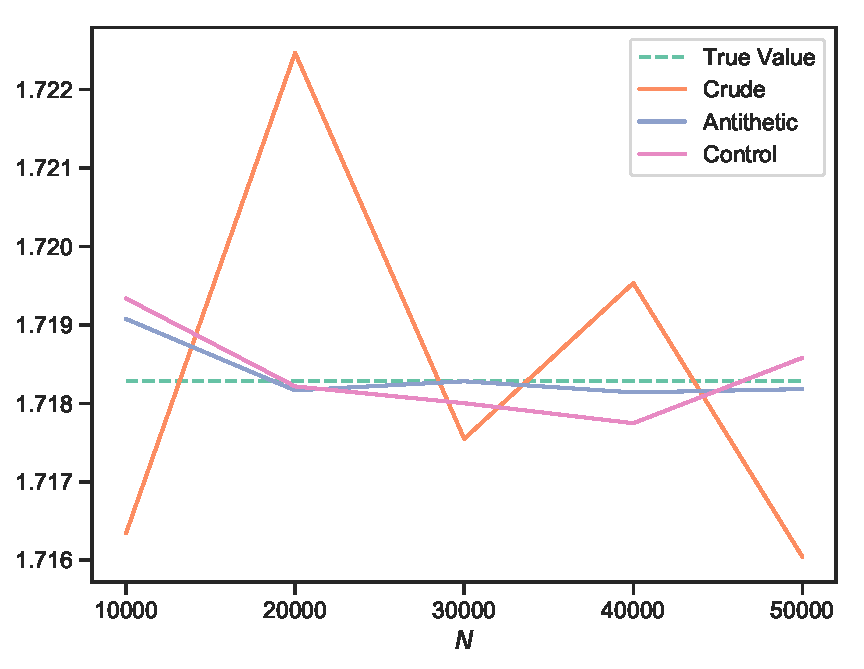
\includegraphics[scale=.93]{../figures/mean.pdf}
                   \label{fig:mean}
                \end{figure}
                As we can see, the variance reduction estimators are very effective at accurately estimating the integral value while reducing the variance considerably,
                while the crude Monte Carlo estimation is comparatively inaccurate and far less consistent.
                The absolute error of each method is visualized in Figure \ref{fig:error} below.
                \begin{figure}[H]
                   \centering
                   \caption{Absolute Errors}
                   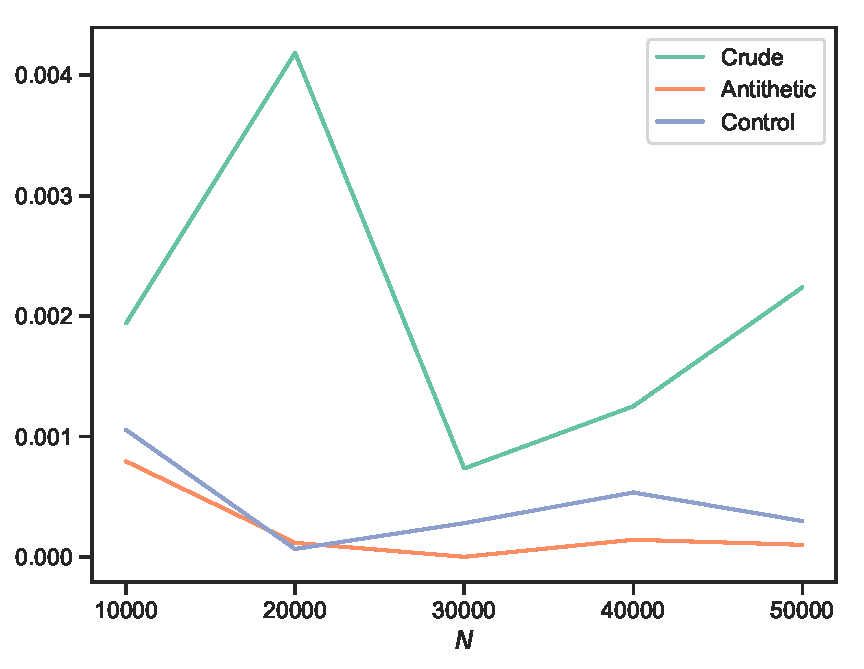
\includegraphics[scale=.93]{../figures/error.pdf}
                   \label{fig:error}
                \end{figure}
                \end{enumerate}
\end{enumerate}
\end{document}
